%%%%%%%%%%%%%%%%%%%%%%%%%%%%%%%%%%%%%%%%%
% Short Sectioned Assignment
% LaTeX Template
% Version 1.0 (5/5/12)
%
% This template has been downloaded from:
% http://www.LaTeXTemplates.com
%
% Original author:
% Frits Wenneker (http://www.howtotex.com)
%
% License:
% CC BY-NC-SA 3.0 (http://creativecommons.org/licenses/by-nc-sa/3.0/)
%
%%%%%%%%%%%%%%%%%%%%%%%%%%%%%%%%%%%%%%%%%

%----------------------------------------------------------------------------------------
%	PACKAGES AND OTHER DOCUMENT CONFIGURATIONS
%----------------------------------------------------------------------------------------

\documentclass[paper=a4, fontsize=11pt]{scrartcl} % A4 paper and 11pt font size

\usepackage[T1]{fontenc} % Use 8-bit encoding that has 256 glyphs
\usepackage{fourier} % Use the Adobe Utopia font for the document - comment this line to return to the LaTeX default
\usepackage[english]{babel} % English language/hyphenation
\usepackage{amsmath,amsfonts,amsthm} % Math packages

\usepackage{lipsum} % Used for inserting dummy 'Lorem ipsum' text into the template

\usepackage{sectsty} % Allows customizing section commands
\allsectionsfont{\centering \normalfont\scshape} % Make all sections centered, the default font and small caps

\usepackage{graphicx}
\usepackage{fancyhdr} % Custom headers and footers
\pagestyle{fancyplain} % Makes all pages in the document conform to the custom headers and footers
\fancyhead{} % No page header - if you want one, create it in the same way as the footers below
\fancyfoot[L]{} % Empty left footer
\fancyfoot[C]{} % Empty center footer
\fancyfoot[R]{\thepage} % Page numbering for right footer
\setlength{\headheight}{13.6pt} % Customize the height of the header

\numberwithin{equation}{section} % Number equations within sections (i.e. 1.1, 1.2, 2.1, 2.2 instead of 1, 2, 3, 4)
\numberwithin{figure}{section} % Number figures within sections (i.e. 1.1, 1.2, 2.1, 2.2 instead of 1, 2, 3, 4)
\numberwithin{table}{section} % Number tables within sections (i.e. 1.1, 1.2, 2.1, 2.2 instead of 1, 2, 3, 4)

\setlength\parindent{0pt} % Removes all indentation from paragraphs - comment this line for an assignment with lots of text

%----------------------------------------------------------------------------------------
%	TITLE SECTION
%----------------------------------------------------------------------------------------

\newcommand{\horrule}[1]{\rule{\linewidth}{#1}} % Create horizontal rule command with 1 argument of height

\title {	
\normalfont \normalsize 
\textsc{Georgia Institute of Technology, College of Computing} \\ [25pt] % Your university, school and/or department name(s)
\horrule{0.5pt} \\[0.4cm] % Thin top horizontal rule
\huge CX4640: Homework 2 \\ % The assignment title
\horrule{2pt} \\[0.5cm] % Thick bottom horizontal rule
}

\author{Nathan Korzekwa} % Your name

\date{\normalsize\today} % Today's date or a custom date

\begin{document}

\maketitle % Print the title

%----------------------------------------------------------------------------------------
%	PROBLEM 1
%----------------------------------------------------------------------------------------

\section*{Problem 3.5}
``The kind of man who would achieve that end, is at the end of achieving his own ends.'' -- Some Pretentious Moron \\


\subsection*{Part A}
	The answer here is C. We can find this without computing the residual because a few quick multiplications reveals that 
	$\left[\begin{array}{c}
		  -1\\
		   1\\
		   1\\
		   -1
		\end{array}\right]$ is orthogonal to $span(A)$.


%----------------------------------------------------------------------------------------
%	PROBLEM 2
%----------------------------------------------------------------------------------------

\section*{Problem 3.17}
\begin{align*}
	\vec{v} = \vec{a} - \alpha\vec{e}_1 \\
	\alpha = -sign(v_1)\|\vec{v}\| \\
	\vec{v} = \left[\begin{array}{c}
			   3\\
			   1\\
			   1\\
			   1
			\end{array}\right] 
\end{align*}

This can be verified in MATLAB.
%------------------------------------------------

%----------------------------------------------------------------------------------------
%	PROBLEM 3
%----------------------------------------------------------------------------------------

\section*{Problem 3.18}
\subsection*{Part A}
3, since there are 3 non-diagonal columns, and Householder makes each column a ``diagonal'' column by zeroing lower entries.

\subsection*{Part B}
The first column of $A$ becomes $\left[\begin{array}{c}
			   -2\\
			   0\\
			   0\\
			   0
			\end{array}\right]$.

\subsection*{Part C}
This column is untouched by the transformation since after that row has been zeroed, we work on the $n - 1 \times n - 1$ submatrix $A'$.

\subsection*{Part D}
There are 6 Givens rotations required because each rotation zeros one position in the matrix, and there are 6 sub-diagonal non-zero entries in this matrix.


%------------------------------------------------

%----------------------------------------------------------------------------------------
%	PROBLEM 4
%----------------------------------------------------------------------------------------

\section*{Problem 3.28}

\subsection*{Part A}
The product $(I - P_k)(I - P_{k - 1})(I - P_{k - 2}) ...$ can be rewritten as $I - P_{k} - P_{k - 1} - P_{k - 2} + P_{k}P_{k - 1} + P_{k-1}P_{k-2} + P_{k}P_{k-1}P_{k-2} ...$. Since the matrices $P_j for  0 < j \leq k$ are all rank-one matrices with each column being orthogonal to each other, $P^mP^n = 0 for m \neq n$, reducing the expression to $(I - P_k - ... - P_1)$.

\subsection*{Part B}
This is equivalent to the classical Gram-Schmidt procedure because it can be rewritten as:
$$
	a_k - P_1a_k - P_2a_k - ... - P_{k - 1}a_k
$$
This clearly follows the logic behind Gram-Schmidt: you expand to the next dimension an orthogonal basis by subtracting the projection of $a$ on to the current vectors in the basis.

\subsection{Part C}
First, we note that $(I - P)$ yields a projection matrix onto a space orthogonal to the space $P$ projects onto. From this, it is easy to see why it represents the Modified Gram-Schmidt process. In the MGS process, when you build the orthogonal basis of dimension $n$ with $n$ linearly independent vectors, when you add a vector to the basis, you first subtract the component of the vector being added from the remaining vectors to be added. So if we start at $a_1$, no vectors have been added yet, so $a_1$ remains unperturbed. But by the time we get to $a_2$, it has already had the component of $a_1$ subtracted off. Interestingly, subtracting off the component of $a_1$ from $a_n$ for any $n$, is equivalent to projecting the vector $a_n$ onto a space orthogonal to the space spanned by $a_1$. This can be computed with $(I - P_1)$. So by the time you start to add $a_k$, it has already been projected onto spaces orthogonal to $a_1$ thru $a_{k-1}$ respectively, thus yielding: $(I - P_1) ... (I - P_{k-1})a_k$.

\subsection{Part D}
The transformation in Part C is equivalent to the transformation in Part B, as shown in Part A. The formulation shown here is Equivalent to the ones in Part B and C because after one transformation by $(I - P_1 - P_2 ... P_n)$ produces a vector that is orthogonal to ALL of the spaces projected onto by $P_1$ thru $P_n$, and as such, transforming an already transformed vector $\vec{v}$ will result in $P_k\vec{v} = 0$ for all $k$, leaving the only nonzero term in the original formulation to be $I$. As a result, any powers of $m > 1$ are equivalent. 


%------------------------------------------------

%----------------------------------------------------------------------------------------
%	PROBLEM 5
%----------------------------------------------------------------------------------------

\section*{Problem 3.12}

\subsection*{Part A and B}
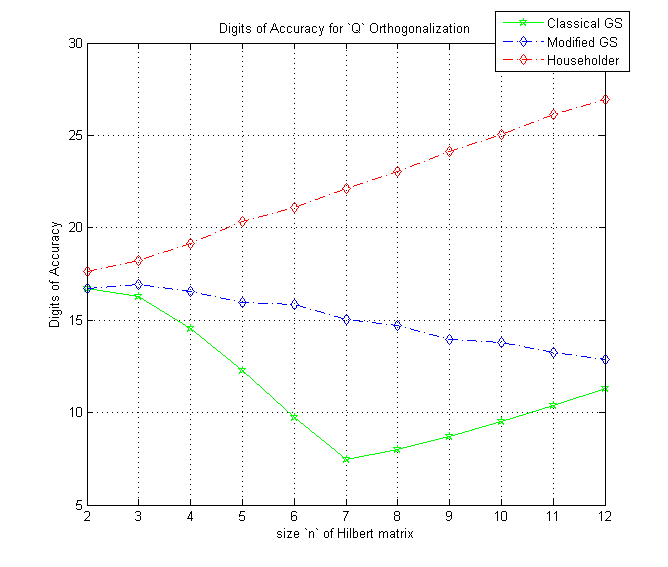
\includegraphics{graph}

In observing the above Graph, it is clear that the accuracy of Householder is the best, followed by the Modified Gram-Schmidt process, followed by the Classical Gram-Schmidt Process. Computationally, they are all bound by the number of columns in the matrix. The Classical and Modified Gram Schmidt processes are equal in run-time since they simply do things in a different order. However, the Modified process allows you to modify the A matrix in-place as it goes along, eliminating the need for separate storage for $Q$. \\

Finally, we have householder -- householder is $O(n^3)$ like G-S, and it also works on sets recursively smaller in size, so the runtime is more or less the same. However, it should be noted that it is more similar to the Modified G-S process in that it can modify the matrix in-place, eliminating the need for extra space for Q.


%------------------------------------------------

\end{document}